% PACKAGES INCLUDED HERE 
% DO NOT NEED TO CHANGE
\documentclass[conference]{IEEEtran}
\IEEEoverridecommandlockouts
% The preceding line is only needed to identify funding in the first footnote. If that is unneeded, please comment it out.
\usepackage{cite}
\usepackage{amsmath,amssymb,amsfonts}
\usepackage{algorithmic}
\usepackage{verbatim}
\usepackage{graphicx}
\usepackage{textcomp}
\usepackage{placeins}
\usepackage{booktabs}

\def\BibTeX{{\rm B\kern-.05em{\sc i\kern-.025em b}\kern-.08em
    T\kern-.1667em\lower.7ex\hbox{E}\kern-.125emX}}
\begin{document}

% AUTHOR NAMES AND TITLE GOES HERE
\title{Food Recognition Software for a Web App}

\author{
\IEEEauthorblockN{1\textsuperscript{st} Heena Khan}
\IEEEauthorblockA{\textit{Computer Science} \\
\textit{Middle Tennessee State University}\\
Murfreesboro, TN\\
hk4h@mtmail.mtsu.edu}
\and
\IEEEauthorblockN{2\textsuperscript{nd} Luis Chunga}
\IEEEauthorblockA{\textit{Computer Science} \\
\textit{Middle Tennessee State University}\\
Murfreesboro, TN \\
lmc6m@mtmail.mtsu.edu}
\and
\IEEEauthorblockN{3\textsuperscript{rd} Steven Sheffey}
\IEEEauthorblockA{\textit{Computer Science} \\
\textit{Middle Tennessee State University}\\
Murfreesboro, TN\\
srs6p@mtmail.mtsu.edu}
\and
\IEEEauthorblockN{4\textsuperscript{th} Matthew Radice}
\IEEEauthorblockA{\textit{Computational Science} \\
\textit{Middle Tennessee State University}\\
Murfreesboro, TN \\
mtr3t@mtmail.mtsu.edu}
\and
\IEEEauthorblockN{5\textsuperscript{th} James Phillips}
\IEEEauthorblockA{\textit{Computer Science} \\
\textit{Middle Tennessee State University}\\
Murfreesboro, TN \\
jmp9q@mtmail.mtsu.edu}
\and
\IEEEauthorblockN{6\textsuperscript{th}  Mason Thieman}
\IEEEauthorblockA{\textit{Computer Science} \\
\textit{Middle Tennessee State University}\\
Murfreesboro, TN\\
mt5e@mtmail.mtsu.edu}
\and
\IEEEauthorblockN{7\textsuperscript{th} Elijah Barbour}
\IEEEauthorblockA{\textit{Computer Science} \\
\textit{Middle Tennessee State University}\\
Murfreesboro, TN \\
enb3r@mtmail.mtsu.edu}
}
\maketitle

% ABSTRACT AND KEYWORDS
\begin{abstract}
 In this work, we classify food images provided by donors using neural networks in order to reduce the amount of work required to donate food. Our software's purpose is to be implemented into an app developed by students at Middle Tennessee State University during the programming event HackMT which allows people to post food that they would like to donate so others may come retrieve it. Image recognition is a computationally heavy task, and training neural networks requires large amounts of memory and extensive run time. This task becomes harder when applied to images that contain noise or similar characteristics to other items within the same category. We process this data using three models called Model 1, Model 2, and Model 3, each taking in 101, 50, and 25 food categories respectively. By applying transfer learning using a pre-trained weights on the NASNet architecture we achieve reasonable accuracy and F1 scores across all of our models. Our best performing model, Model-3, is trained on 25 randomly selected food categories, achieves a top 10 accuracy of 81\% and an F1 score of 52\% averaged over 5 folds. We believe these results are sufficient for the target food identification feature. 
\end{abstract}


\begin{IEEEkeywords}
food detection; image recognition; convolutional neural networks
\end{IEEEkeywords}

% SECTIONS
\section{Introduction}

Zhengxia Dou et. al. show that consumers waste approximately 41 million metric tonnes of food per year~\cite{Food_Waste}. By implementing this neural network into the app, we aim to prevent food wastage and help provide food to someone who needs it. A proposed solution to this problem is an app developed by students at Middle Tennessee State University, which enables users to donate food which would otherwise go to waste. However, this app requires manual input of information about the donated food, which makes the donation process tedious.

In order to reduce the amount of work required to donate food, we propose the use of a Neural Network (NN) to automatically classify pictures of donated food. This reduces the work required to donate food on the app, by automatically classifying images of donated food, and recommending potential labels to the donor.



\section{Background}

Lukas Bossard, Matthieu Guillaumin, and Luc Van Gool introduce the Food-101 dataset, and explore the food image classification problem~\cite{mainRef}. The Food-101 dataset~\cite{dataset} consists of 101 categories of popular foods with each category containing 1000 images. Of each category's 1000 images, 750 of these images have not been cleaned and contain color and categorical noise. They used a random forest to identify unique aspects of different classes simultaneously rather than one at a time so that the network could share information about each class as it was being trained. Their model achieved an average accuracy of 50.76\% over 101 classes \cite{mainRef}. With the resources we had available for testing this project, we branched from their article and focused on using color and texture as our primary features combined with a transfer learning model using CNN's. As discussed previously, training a neural network to learn image recognition is a computationally heavy task and it requires a very large dataset to perform well. In order to reduce this cost, many articles use Transfer Learning in place of training a model from start to finish. 

Computer Vision (CV), or image recognition, begins by breaking down images into pixels. These pixels can be converted into numerical information representing color, shape, texture, and other features \cite{Tlearning}. While one pixel of an image may not be able to give much information, splitting the image into multiple sections by using Convolutional Neural Networks (CNN) allows us to store that information and attribute it to a specific label. 

 CNNs are extremely useful in the process of image recognition. In \cite{CNN} Panu Asikanius states, ``the task of image recognition proves to be too demanding for a regular neural network simply because of the sheer number of parameters. A small RGB image file of 300×300 pixels accumulate to a weight vector of length 270000. Adding several layers with full connectivity quickly adds up to an astronomical number of parameters.'' CNNs reduce a model's parameter count exponentially by taking advantage of the two dimensional form of images. By specifying the height, width, and depth of a convolutional kernel, we can gather information in windows rather than processing all the information provided by an image at one time. After being processed by a convolutional layer, the resulting output is frequently passed into pooling layer that reduces the computational resources needed for processing. 

The use of Transfer Learning is best defined by Yin Zhu where they describe it as the learning of features that can be attributed to a range of common datasets~\cite{Tlearning}. In the case of image datasets, useful features such as textures, shapes, and color can be learned from a multitude of images that are not focused within a singular domain. This knowledge can then be applied to a NN that is being trained on a different category, such as food, and have its parameters or parameters of additional layers tuned to fit the new domain.
 
 While there are a multitude of models pre-trained on ImageNet, we have chosen to use NASNet as a basis for our model. ImageNet provides on average 500–1000 images to illustrate each synset in WordNet. Images of each concept are quality-controlled and human-annotated. ImageNet, offers tens of millions of cleanly sorted images~\cite{ImageNet}. NASNet is an classification model developed for ImageNet classification \cite{NASNetDef}. But even with the pre-trained model there is still a major issue with overfitting. Y. Zhang, L. Wu, and S. Wang propose the use of k-fold cross validation in the hopes of circumventing this overfitting problem because it moves through the training and validation data $K$ times and averages the results between each fold while training.  
 

\section{Methods}
\subsection{Mathematical Execution}
One medium that we can use to represent our processes logically is the already-established foundations of mathematics. For example, the net input for a unit can be “folded” into a single value, $net_{j}$, which weights the activation of the sending neuron $x_{i}$ by the strength of the synaptic connection between i and j, $w_{ij}$. The sum of all weighted activations into a unit plus a bias weight, $w_{0}$, is the total net input. This can be represented in the equation below:
\begin{equation}
net_{j} = w_{0} + \sum_{i = 1}^{n}{x_{i}w_{ij}}\label{eq}
\end{equation}
This is an example of a way that mathematics is an adequate measure in which neural networks can be represented. Naturally, we learn more about an object or process by making incremental updates to the subject in our minds. Since artificial neural networks mimic natural neural networks, we need a way to represent incremental changes within our artificial neural network. Calculus is the mathematics of change, so the logical conclusion is to use Calculus to represent change within our artificial neural network. 
We used Rectified Linear Units (ReLU) as our activation function for a few of the hidden layers in our CNN. ReLU can be represented by the following equation:
\begin{equation}
f(x) = \mathrm{max}(0,x)\label{eq}
\end{equation}
where x is an input value. ReLU was chosen as the activation function for many hidden networks because of its simplicity in computation as opposed to others like the hyperbolic tangent (tanh) and sigmoid activation functions that are more computationally demanding. By keeping computation simple it speeds up training time. Because our objective is to classify pictures, we also used softmax, an activation function commonly used for the classification of multiple tags.
\subsection{Theoretical Execution}
The inspiration for building and implementing artificial neural networks for Artificial Intelligence stems from biological foundations. Although Artificial Neural Networks function different from Natural Neural Networks, the mathematical developments in the field were all inspired by natural processes. Knowing that this NN was influenced by natural brain processes, we can then look at the neurons roughly as an electrical processing system and keep that in mind as we are making our network. Base the mathematical developments we are attempting to create a NN with tools such as Keras and TensorFlow that could train a model to recognize food images.


\subsection{Practical Execution}
 
In the first attempt, we developed a model using the pre-train model MobileNet as our simple base net. On a small dataset, the accuracy was good, but when we implemented it with the entire dataset, it did not give us good results. Then we tried a couple of MobileNet models such as MobileNetV2 and NASNetMobile. The reason that we stick to a Mobile network is that it's very resource consuming to train a whole massive Imagenet model.

\subsection{Model Architecture}
Our models accept an image of size 224 x 224 x 3 and output a probability vector of size $N$, where $N$ is the number of classes the model is trained to consider. Our primary model uses a pre-trained NASNetMobile model as its base. We removed the final layers and added a max-pooling layer, a dense layer of varying size $N$, it is 101 for Model 1, 50 for Model 2 and 25 for Model 3, and a dropout layer with parameter 0.5. This architecture can be seen in Figure~\ref{fig:model}. We have not included NasNet architecture in our model summary because NasNet is a massive model with too many convolutional layers, max-pooling layers, and a dense layer.

% CREATES IMAGE FIGURE
\begin{figure}[htbp]
\centerline
{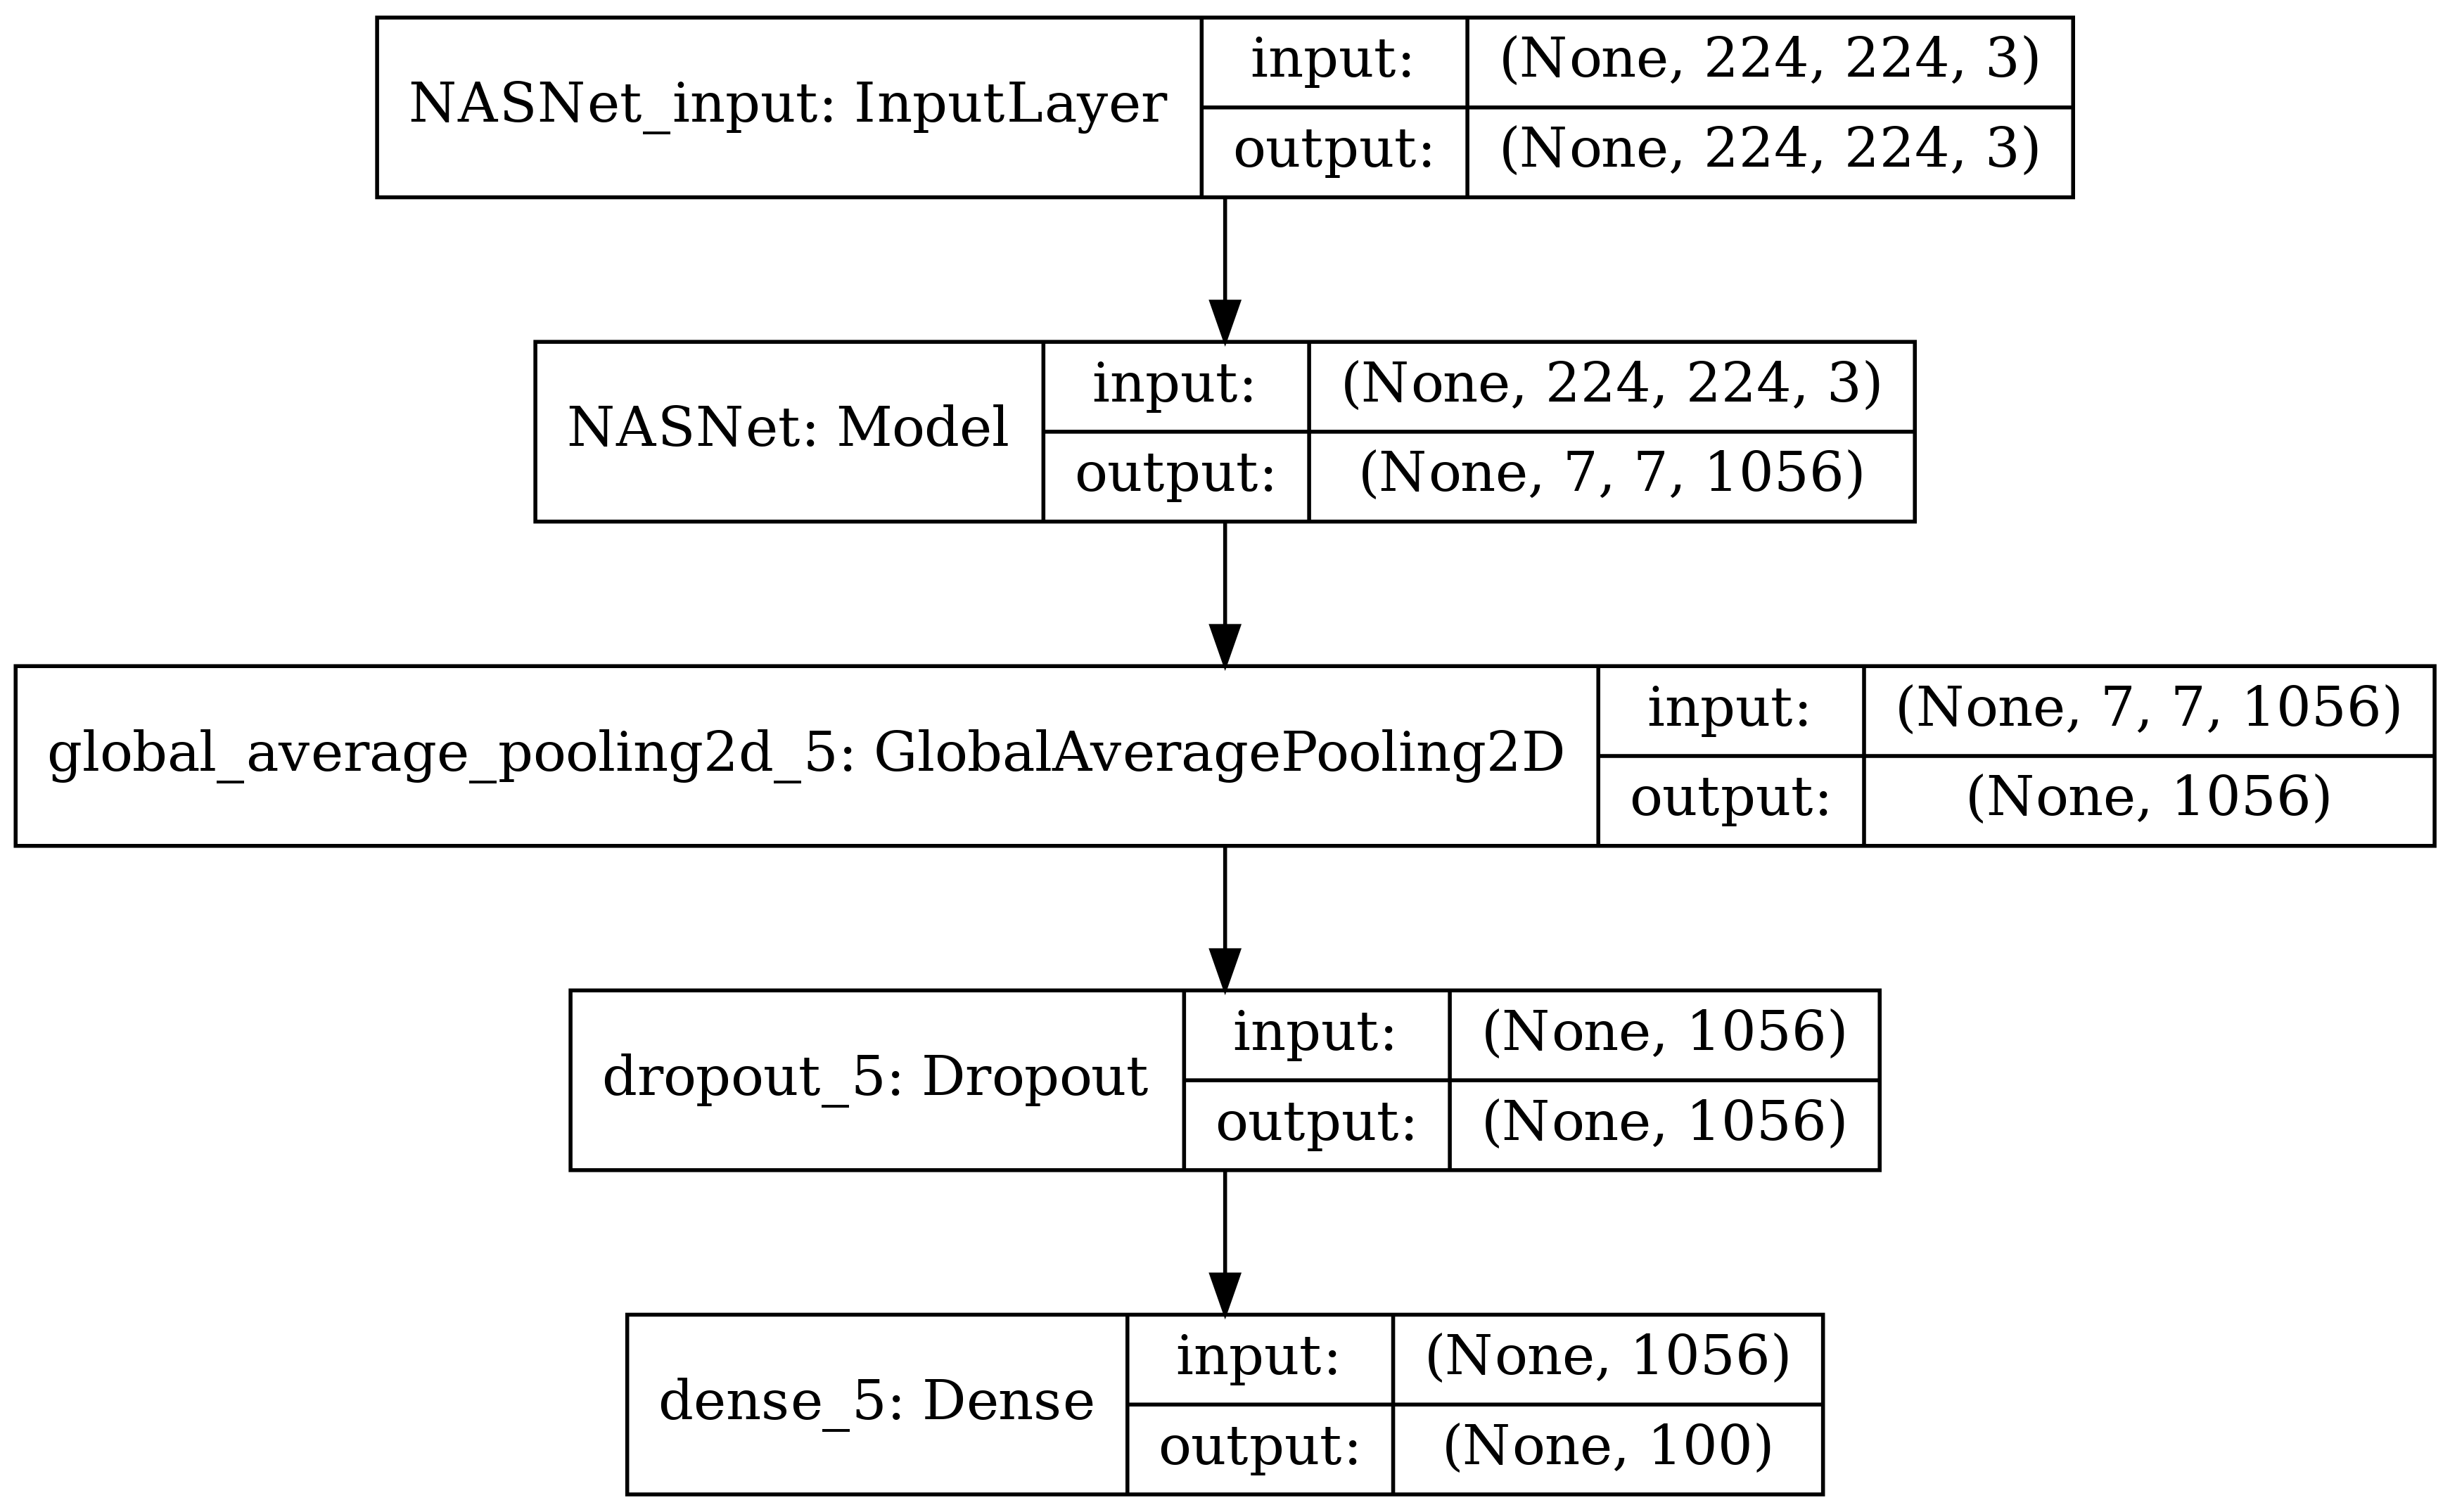
\includegraphics[width=\columnwidth]{images/model.png}}
\caption{Model Architecture}
\label{fig:model}
\end{figure}


For our models, we used Keras's \texttt{ImageDataGenerator} to rescale, rotate, shift, and flip the images. Modern image recognition can require heavy amounts of memory and processing power. Additionally, the training of these neural networks requires large amounts of data. Loading training data into memory can be impossible when the dataset is large. One way of solving this issue is through the use of Keras's \texttt{ImageDataGenerator}. This helps reduce the strain on the system from trying to load what could be thousands or hundreds of thousands of images all at once. The data generator also provides methods for image pre-processing, such as resizing images, normalizing pixel values, and augmenting the dataset with transformations such as translation or rotation. These are useful features because the images in the Food 101 dataset are saved in a variety of resolutions.

In this research, we created three models. All three models had the same architecture mentioned above but different number of classes. Model 1 was trained on 101 food categories. Model 2 was trained on 50 food categories, and Model 3 was trained on 25 food categories. Our dataset consists of 101 food categories; for Model 1, we used the entire dataset. For Model 2, we randomly selected 50 food categories and trained our model on it, and for Model 3, we randomly selected 25 food categories and trained our model on it. For each of our model, we have three different accuracy's for top 1, top 5, and top 10 predictions.

Then, we used the k-fold cross-validation to estimate our accuracy. For the three models, we used an average of 5-fold for each model. For each fold, We randomly split the dataset into four parts for training and one part for testing. Also, we use a 10\% of our training dataset for validation. After each k-fold is run, we evaluate and predict our model to compare the top 1, top 5, and top 10 accuracy.

\section{Results}
We first created  Model 1 that is trained on 101 classes. Even on changing different architecture, the average 5-fold accuracy of Model 1 was no better than 22\%, and it was essential to have a better accuracy since we had to deploy our model to a Web app. So we created the other two other models, Model 2 and Model 3, with 50 and 25 classes, respectively. We found that though the accuracy of Model 2 and Model 3 was better than Model 1, it was still not identifying most of the images. We also noticed that our Model 1, though, doesn't recognize a lot of food categories as top 1, but most of them are under the top 10 prediction out 101 categories. So for every model, we calculated top1, top5, and top10 accuracy's. Since our Model 1 could identify most of the images within Top 5 and more of the images within Top 10. We deployed Model 1 into our Web app.

\FloatBarrier
The Accuracy of our models, averaged over 5 folds for Top-1 class, Top-5 classes and Top-10 classes for all our three models is displayed in Table :~\ref{tab:accuracy_table}
% CREATES Table
\FloatBarrier
\begin{table}[!htbp]
\caption{Accuracy of our models, averaged over 5 folds}
\label{tab:accuracy_table}
\resizebox{\linewidth}{!}{%
\begin{tabular}{ccccc}
\toprule
                     & Classes & Top 1 & Top 5 & Top 10 \\ \midrule
Model 1 & 101 & 22.23\%  &   42.31\%    &     52.56\%   \\
Model 2 &  50  & 34.30\%  & 59.52\%      &     70.99\%   \\
Model 3 &  25  & 41.37\%  &   69.17\%    &    80.68\%    \\ \bottomrule
\end{tabular}%
}
\end{table}

\FloatBarrier
% CREATES IMAGE FIGURE
\begin{figure}[!htbp]
\centerline
{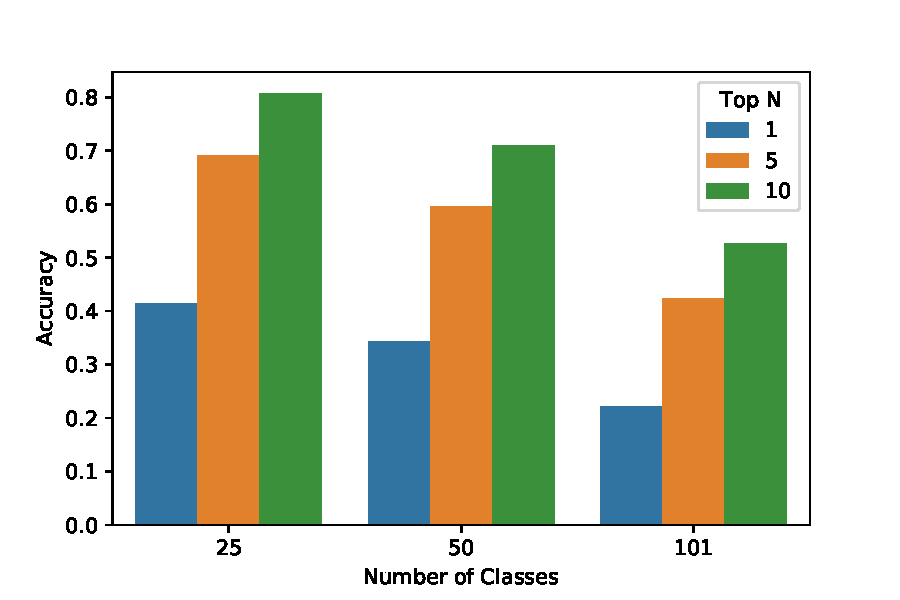
\includegraphics[width=\columnwidth]{images/accuracies.pdf}}
\caption{Top N accuracy values across all 3 models}
\label{fig:accuracies_barchart}
\end{figure}

\FloatBarrier
Model 1 being trained on 101 classes has an accuracy of 0.2223 with f1 score of 0.3319. 
Figure ~\ref{fig:acc_loss_101} Represents the accuracy plot for our Model 1.
 
% CREATES IMAGE FIGURE
\begin{figure}[h]
\centerline
{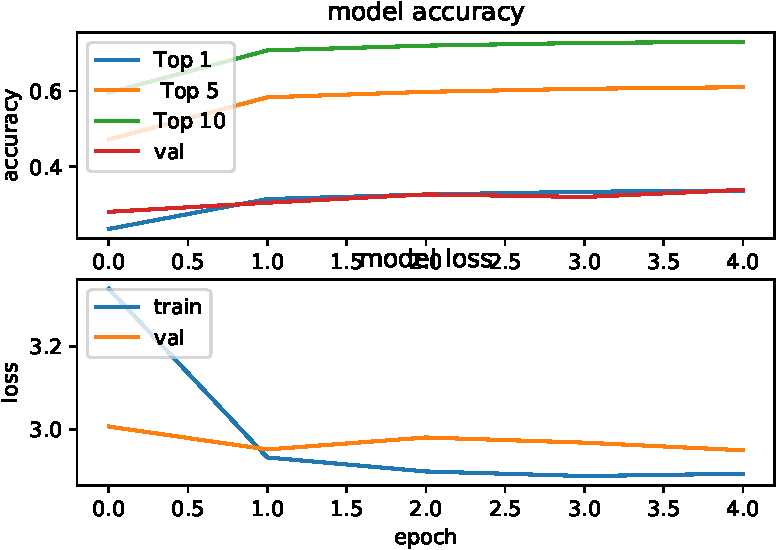
\includegraphics[width=\columnwidth]{images/acc_loss_101-cropped.pdf}}
\caption{Top1, Top5 and Top 10 accuracy of Model 1 }
\label{fig:acc_loss_101}
\end{figure}

\FloatBarrier
Model 2 being trained on 50 random classes has an accuracy of 0.3430 with f1 score of 0.4322.
Figure ~\ref{fig:acc_loss_50} Represents the accuracy plot for our Model 2.
% CREATES IMAGE FIGURE
\begin{figure}[h]
\centerline
{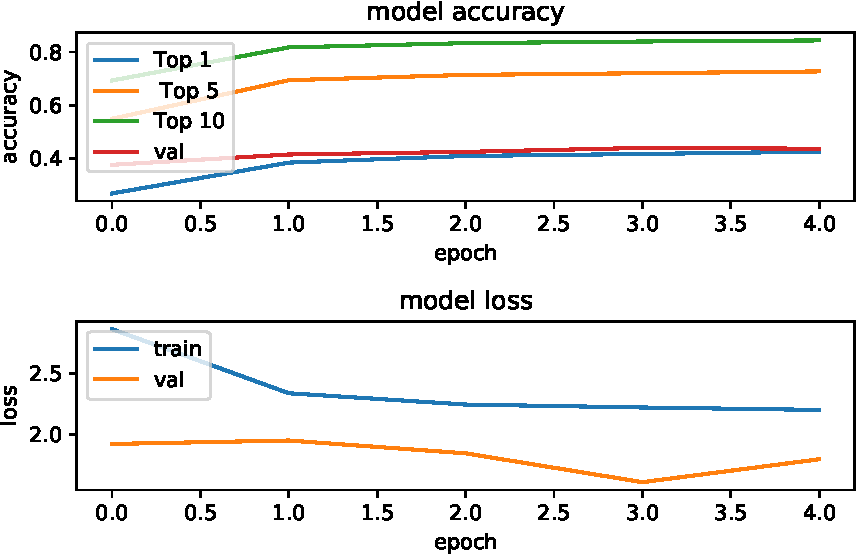
\includegraphics[width=\columnwidth]{images/acc_loss_50-cropped.pdf}}
\caption{Top1, Top5 and Top 10 accuracy of Model 2 }
\label{fig:acc_loss_50}
\end{figure}

\FloatBarrier
Model 3 being trained on 25 random classes has an accuracy of 0.4137 with f1 score of 0.5203. 
Figure ~\ref{fig:acc_loss_25}  Represents the accuracy plot for our Model 3.
% CREATES IMAGE FIGURE
\begin{figure}[h]
\centerline
{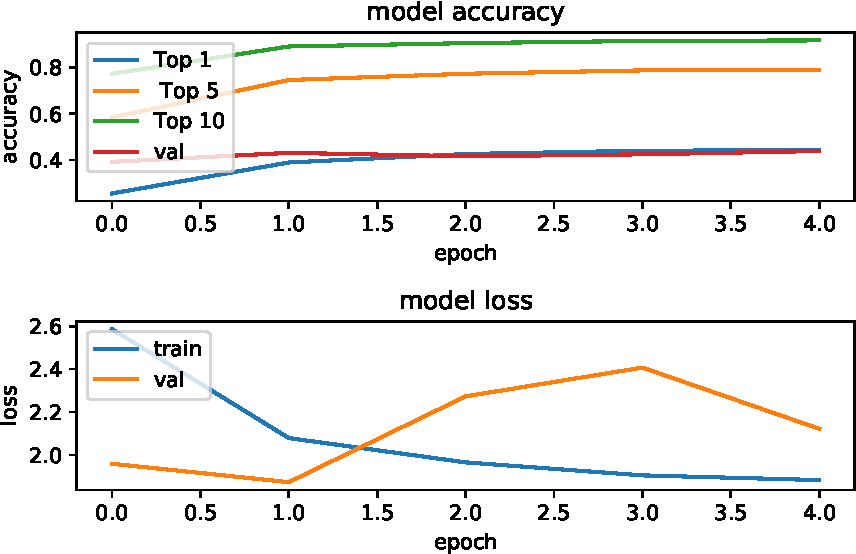
\includegraphics[width=\columnwidth]{images/acc_loss_25-cropped.pdf}}
\caption{Top1, Top5 and Top 10 accuracy of Model 3}
\label{fig:acc_loss_25}
\end{figure}


\FloatBarrier
We have generated a false-positive rate (FPR), true-positive rate (TPR) matrix, to identify our models precision. The diagonal represents (predicted label = actual label) where we want our maximum count to be. However, there are several misclassifications. Figure ~\ref{fig:CM_101} represents the FPR and TPR matrix for Model-1. Figure ~\ref{fig:CM_50} represents the FPR and TPR matrix for Model-2, and Figure ~\ref{fig:CM_25} represents the FPR and TPR matrix for Model-3.

% CREATES IMAGE FIGURE
\begin{figure}[!htbp]
\centerline
{\includegraphics[width=\columnwidth]{images/Conf_101-cropped.pdf}}
\caption{TPR and FPR confusion matrix for Model 1}
\label{fig:CM_101}
\end{figure}
In Figure ~\ref{fig:CM_101}, We have a light diagonal, that represents our true-positive. Also, we can see there are several misclassifications/false-positives throughout our matrix.

\FloatBarrier
Figure~\ref{fig:CM_50}  Represents the confusion matrix for our Model 2.
% CREATES IMAGE FIGURE
\begin{figure}[!htbp]
\centerline
{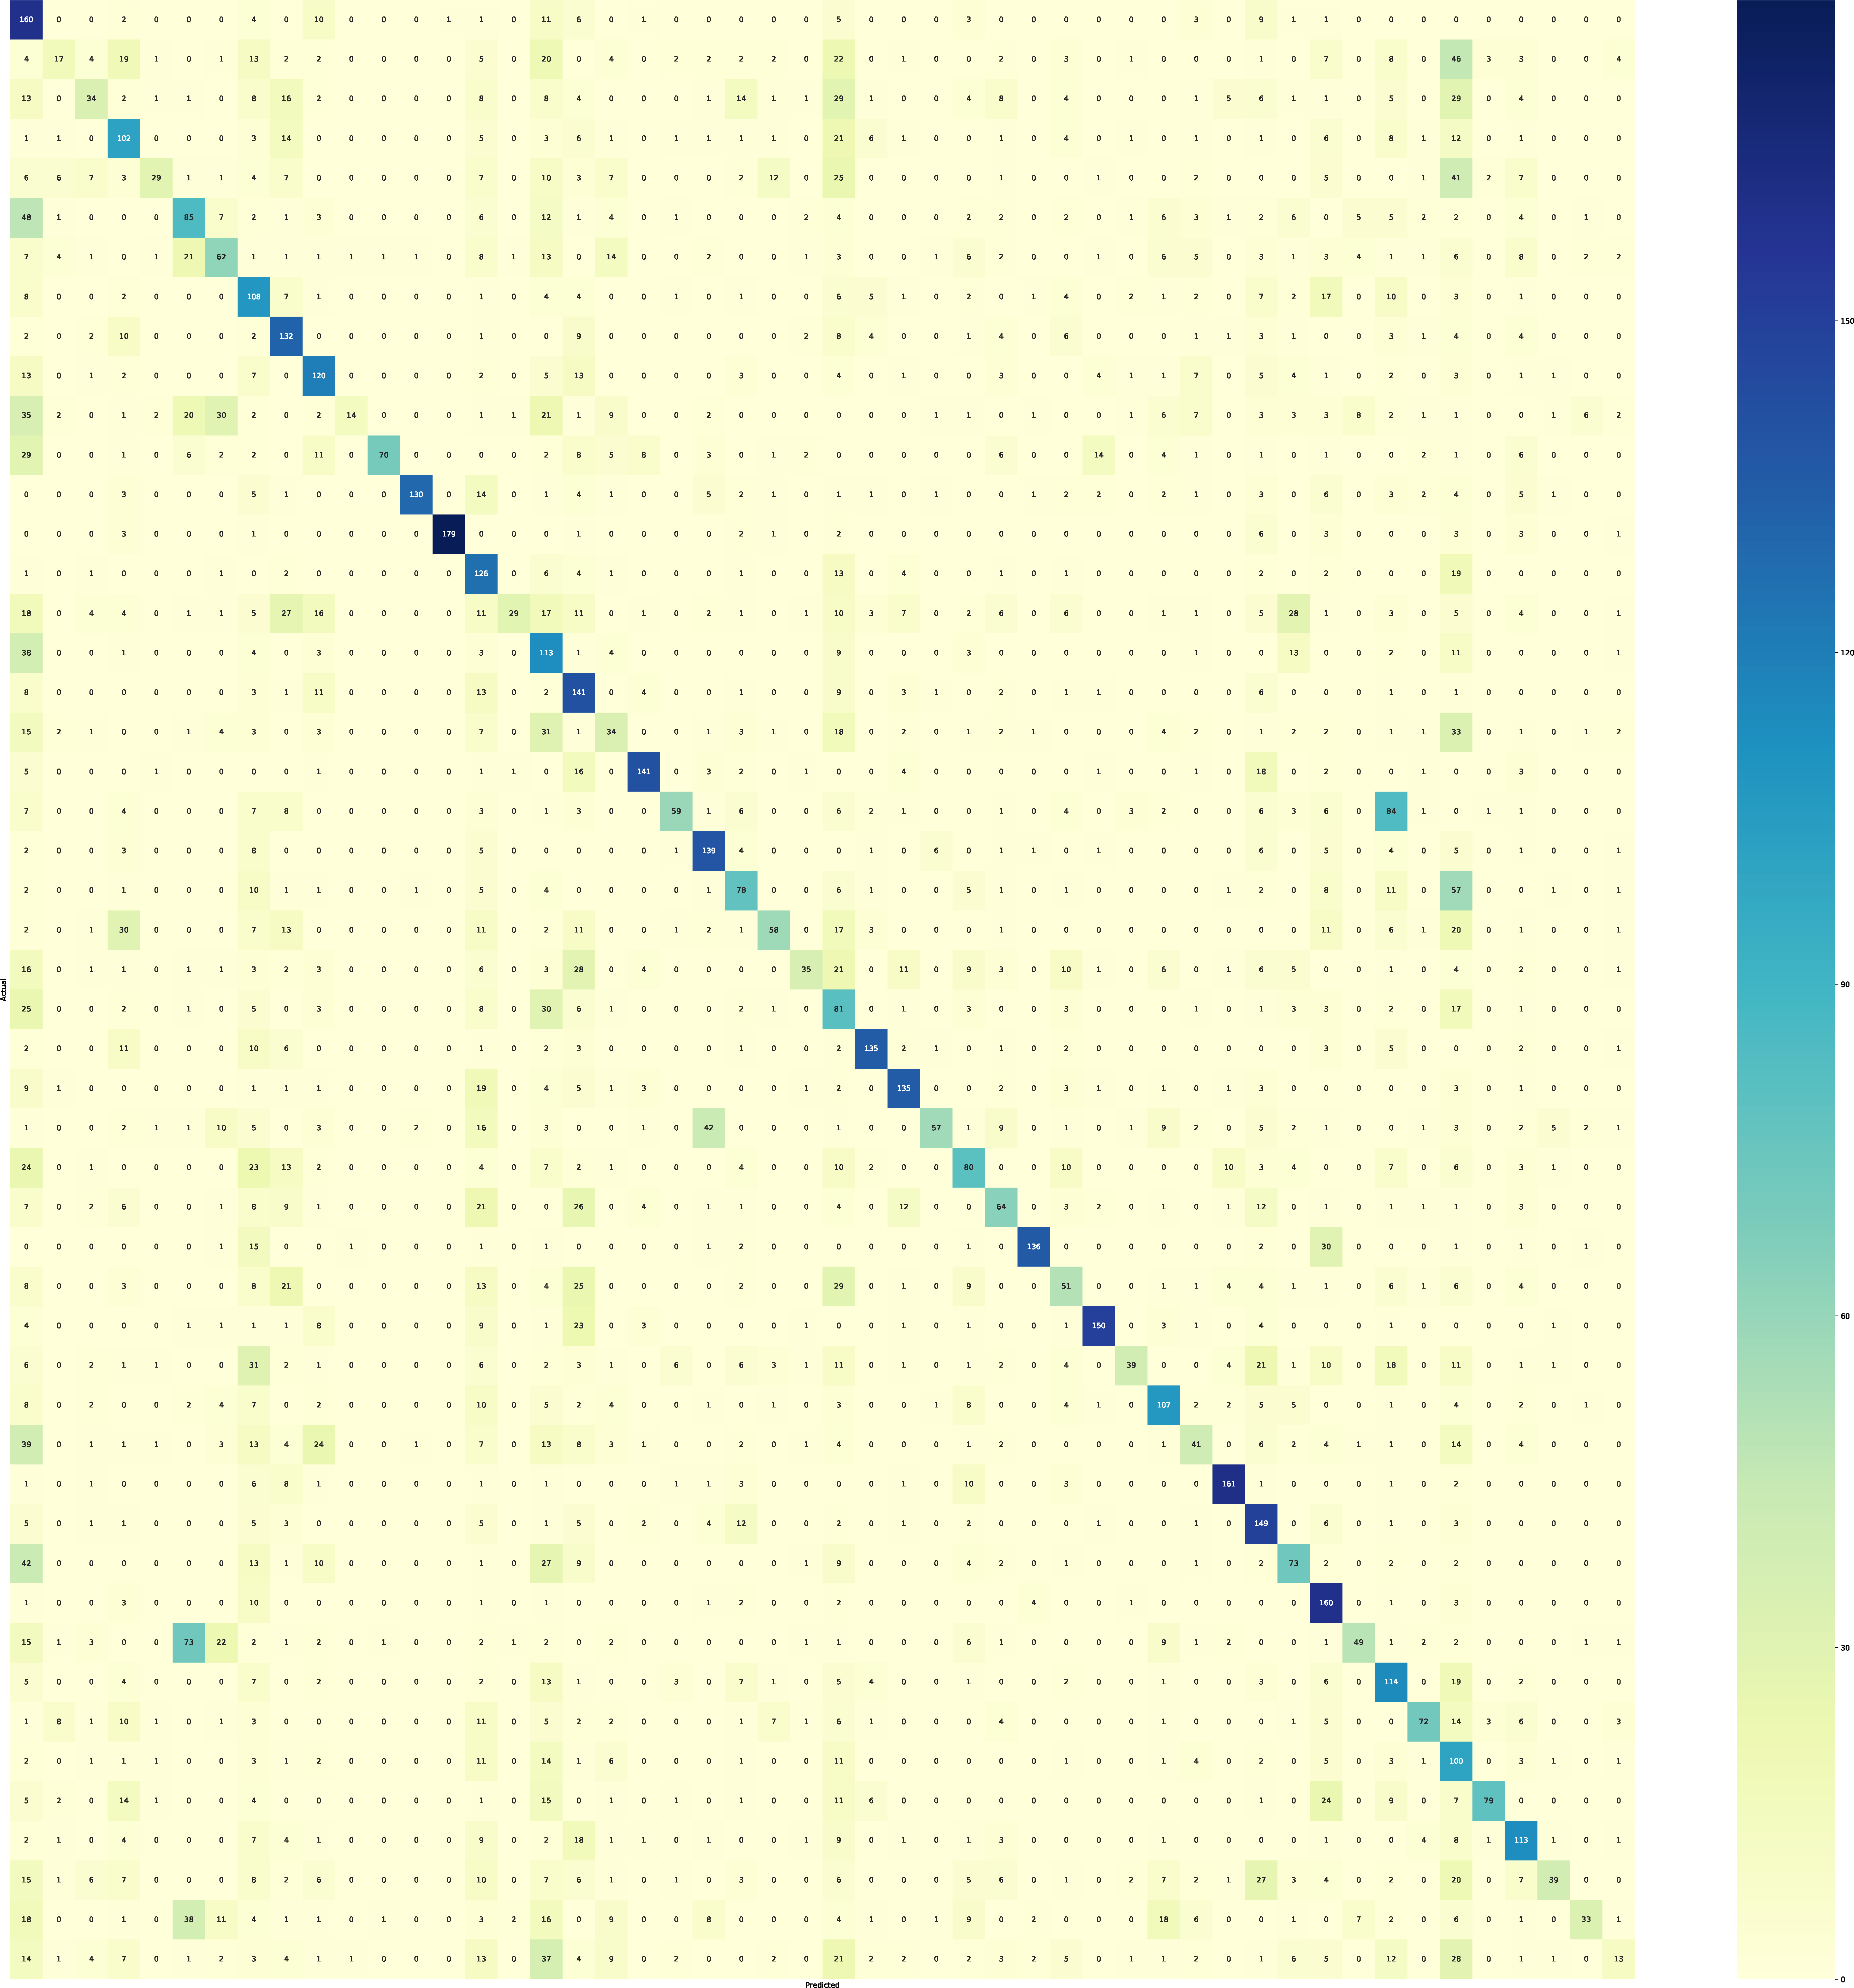
\includegraphics[width=\columnwidth]{images/Conf_50-cropped.pdf}}
\caption{TPR and FPR confusion matrix for Model 2}
\label{fig:CM_50}
\end{figure}
In Figure ~\ref{fig:CM_50}, We have a slightly darker diagonal, that represents our true-positive. We can see that some classes were identified better than the other. Also, there is some improvement in our misclassifications/false-positives rate. 

\FloatBarrier
% CREATES IMAGE FIGURE
\begin{figure}[!htbp]
\centerline
{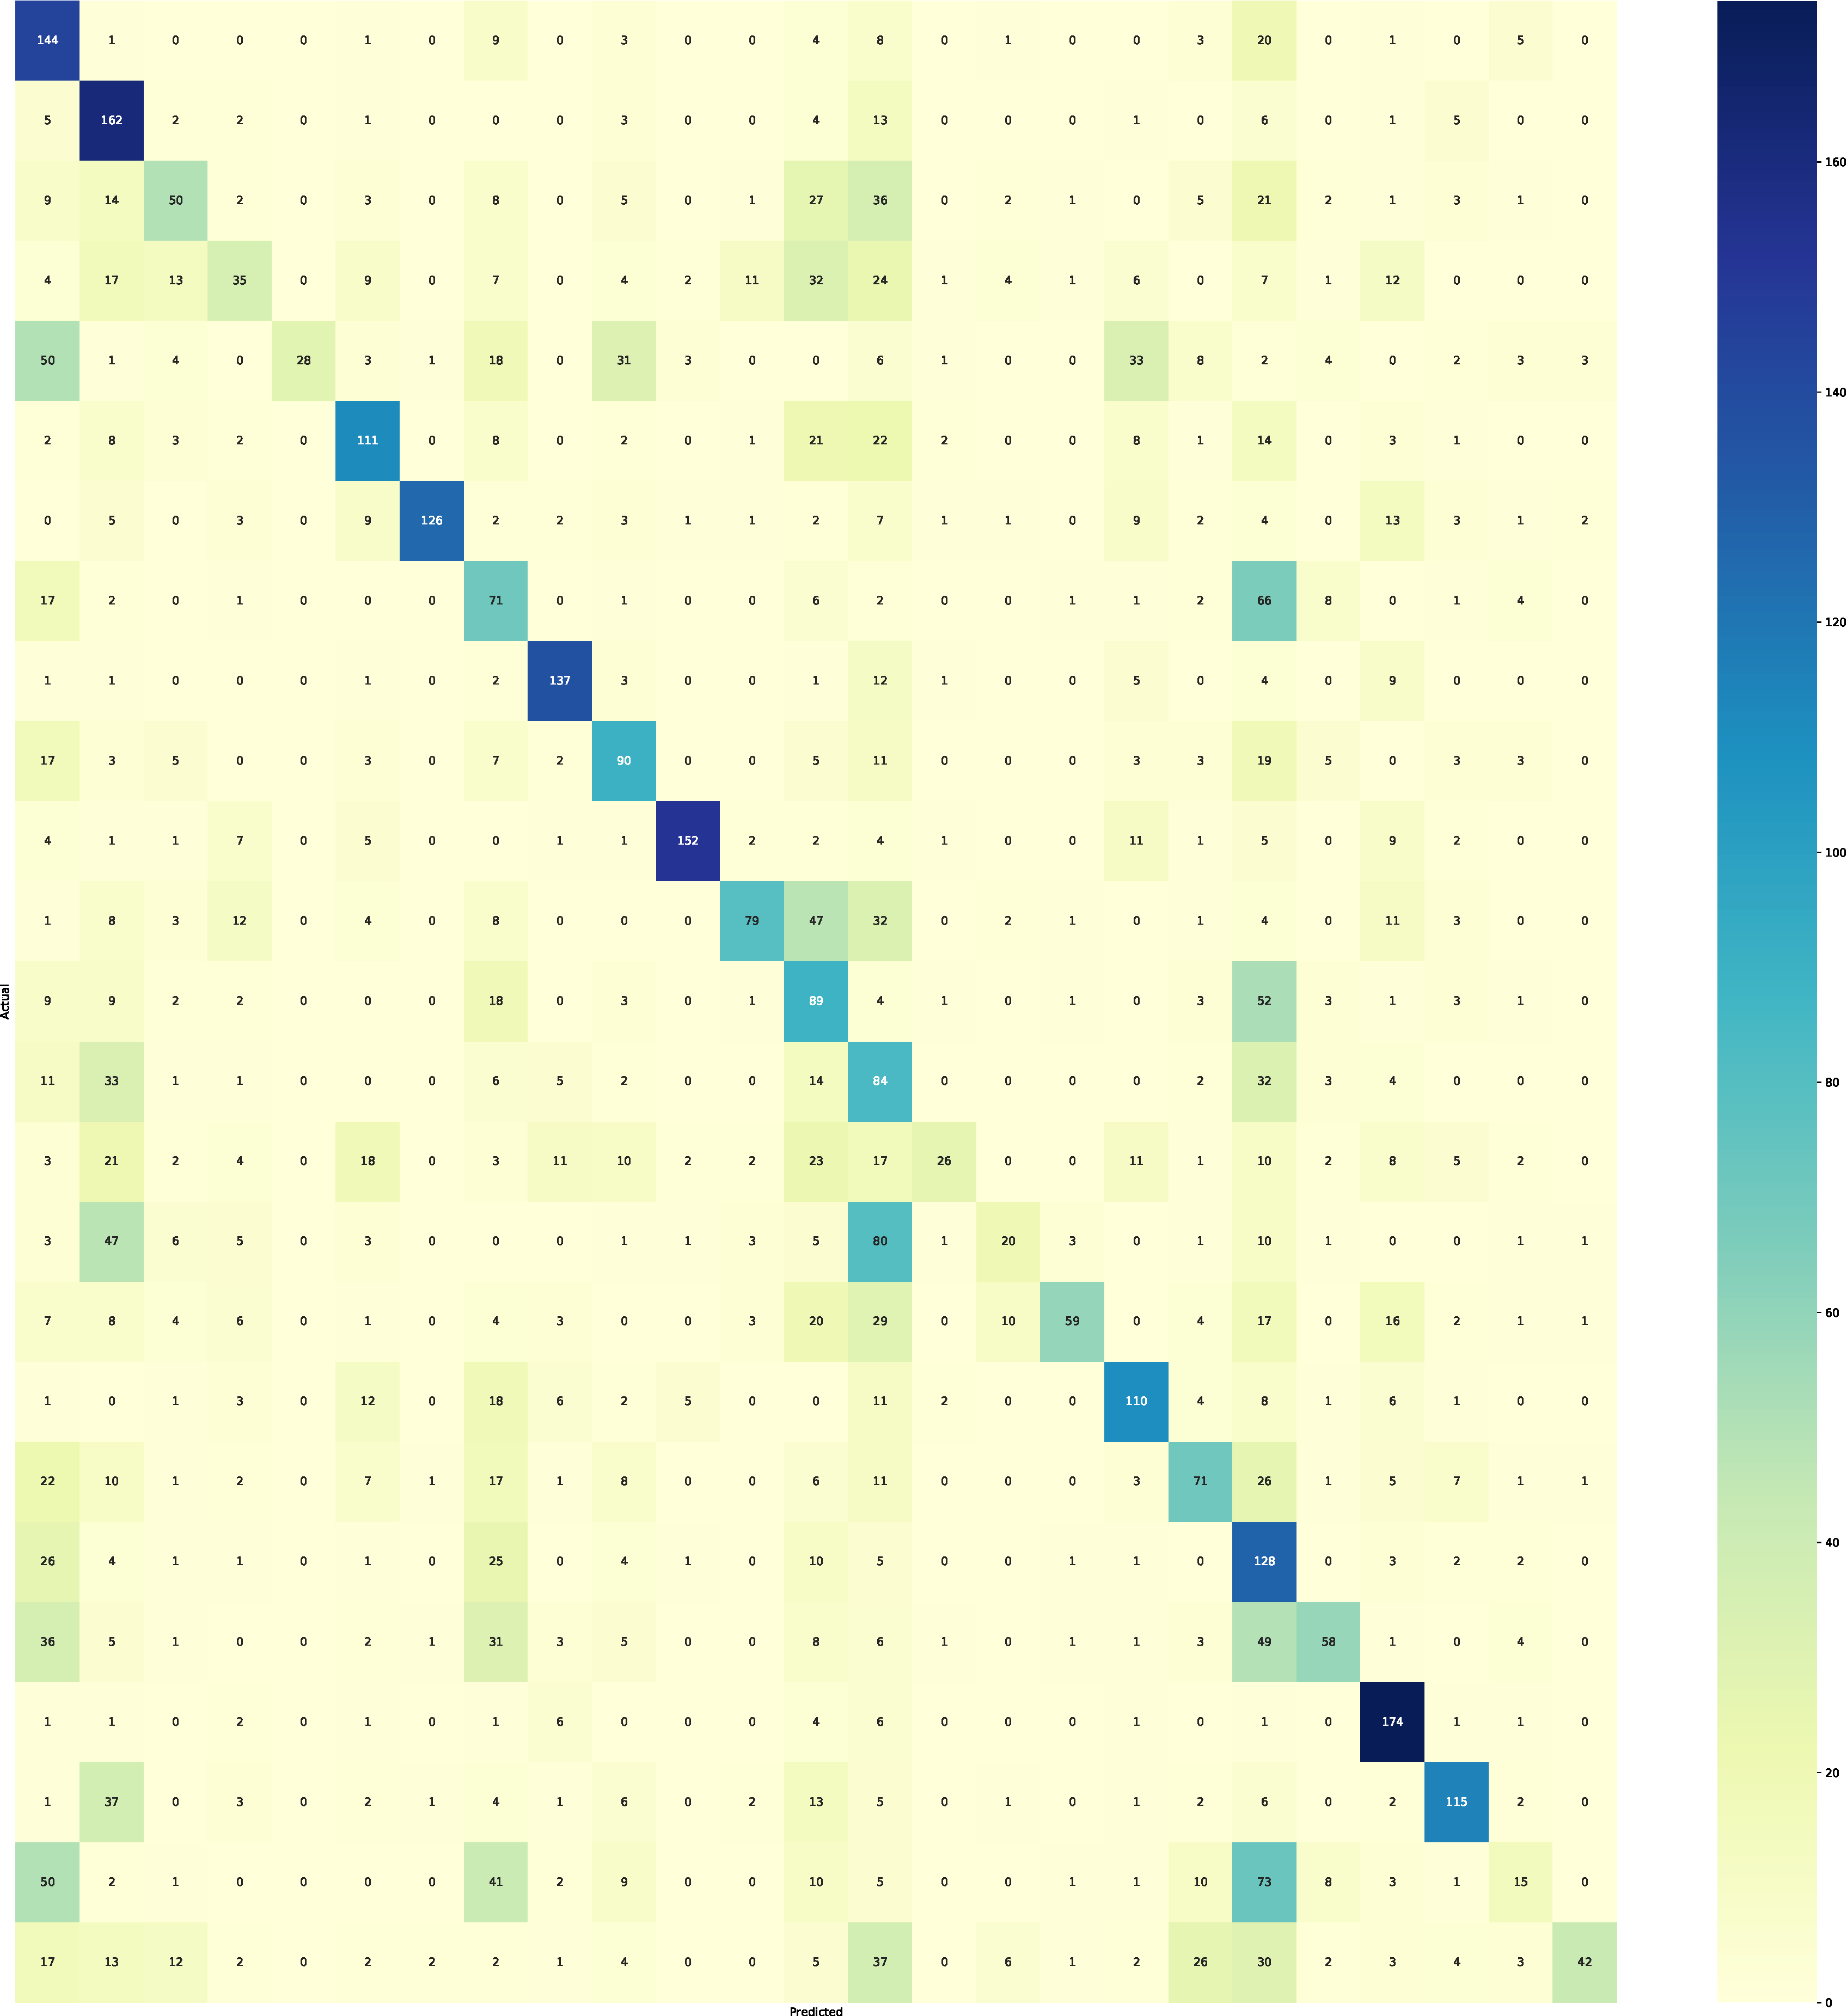
\includegraphics[width=\columnwidth]{images/Conf_25-cropped.pdf}}
\caption{TPR and FPR confusion matrix for Model 3}
\label{fig:CM_25}
\end{figure}
On the basis of accuracy Model 3 is our most efficient model.
In Figure ~\ref{fig:CM_25}, We have a darker diagonal, that represents our true-positive. We can see that half of the classes were identified better than the other half. Also, there is some improvement in our misclassifications/false-positives rate. 

\section{Discussion}
Training a neural network from scratch is not an easy task, especially when training on images classifications, significant architecture engineering is needed. Our model leans heavily on a pre-trained NASNet which was built by designing a search space so the complexity of the architecture is independent of the depth of the network and size of input images\cite{zoph2017learning}. The approach used convolutional networks that were composed of convolutional "cells" with identical structure but with different weights. Searching for the best convolutional architecture was reduced to the best cell structure. According to \cite{zoph2017learning} this has two main benefits: it is much faster than searching the entire network architectures and the cell itself is more likely to generalize to other problems. Being able to generalize to other problems is a feature we will utilize for our project. 

To put the training used to achieve this network into perspective, the controller RNN used in \cite{zoph2017learning} employed a global work-queue system for generating a pool of child networks that consisted of 500 GPUs and took over 4 days to yield several candidate convolutional cells. This network was then trained on CIFAR-10 data-set and due to the network being able to generalize, the best convolutions cells were used and trained all ImageNet model weights from scratch. 

Our network uses these pre-trained weights from the ImageNet data set to start from, as achieving such weights is outside the scope of this project and available resources. The ImageNet data set does not focus on food but contains a broad range of topics in 1,000 categories of 1.2 million images. This means our network will need to adjust its weights from a broad spectrum of classes to a more narrow spectrum of classes. The network is also contending with data that contains a lot of variety and noise within each class, not to mention miss-labeled data which can also lead to challenges when searching for specific weighs for our data. As shown in Table 1, our fine-tuning of the network and use of k-fold cross validation allowed us to achieve solid results achieving from 50\% up to 80\% when returning the top 10. When testing our 3 models, accuracy increases as the number of classes decreases. This is due to the network being able to learn and classify fewer classes more accurately.

As shown in Figures 3, 4, and 5, all 3 models display similar learning curve but achieve different accuracy's depending on how many classes are used in each model. There is close to a 40\% increase from top 1 to top 10. Predicting the correct food type 100\% of the time is of course ideal, but not necessary. The program would still be able to save the user time by providing a list of either the top 5 or the top 10 choices to choose from. This also allows for the user to have some control of the final choice if there is any discrepancies in the output and the user wants to override the networks choice. The top 5 or top 10 will add that functionality organically by simply displaying the food items that share some details in common.

When it comes to the number of classes the network examines there is also a trend. As the number of classes decreases the accuracy increase is close to 20\% from 101 to 25 classes. Thinking about how these networks find different features in the images using convolution, it seems that a logical conclusion is that the fewer the images the less features that will overlap and possibly return the wrong food item. So when providing the network 101 different classes each containing 1000 images there is more likely features that will overlap, compared to 25 classes, where the likely hood of features being different will increase.

After generating our convolution neural network model we trained on 101 food items (classes). We created a front end web application using HTML, CSS, and JavaScript that accepts an image and sends the image to our Keras model being hosted by Flask. The Keras model then returns the top 1, top 5, and 10 predictions for the image. By clicking on one of the predictions, the user can pick the food they are serving. Figure:~\ref{fig:fig2} represents the front end of our web page.

% CREATES IMAGE FIGURE
\FloatBarrier
\begin{figure}[htbp]
\centerline
{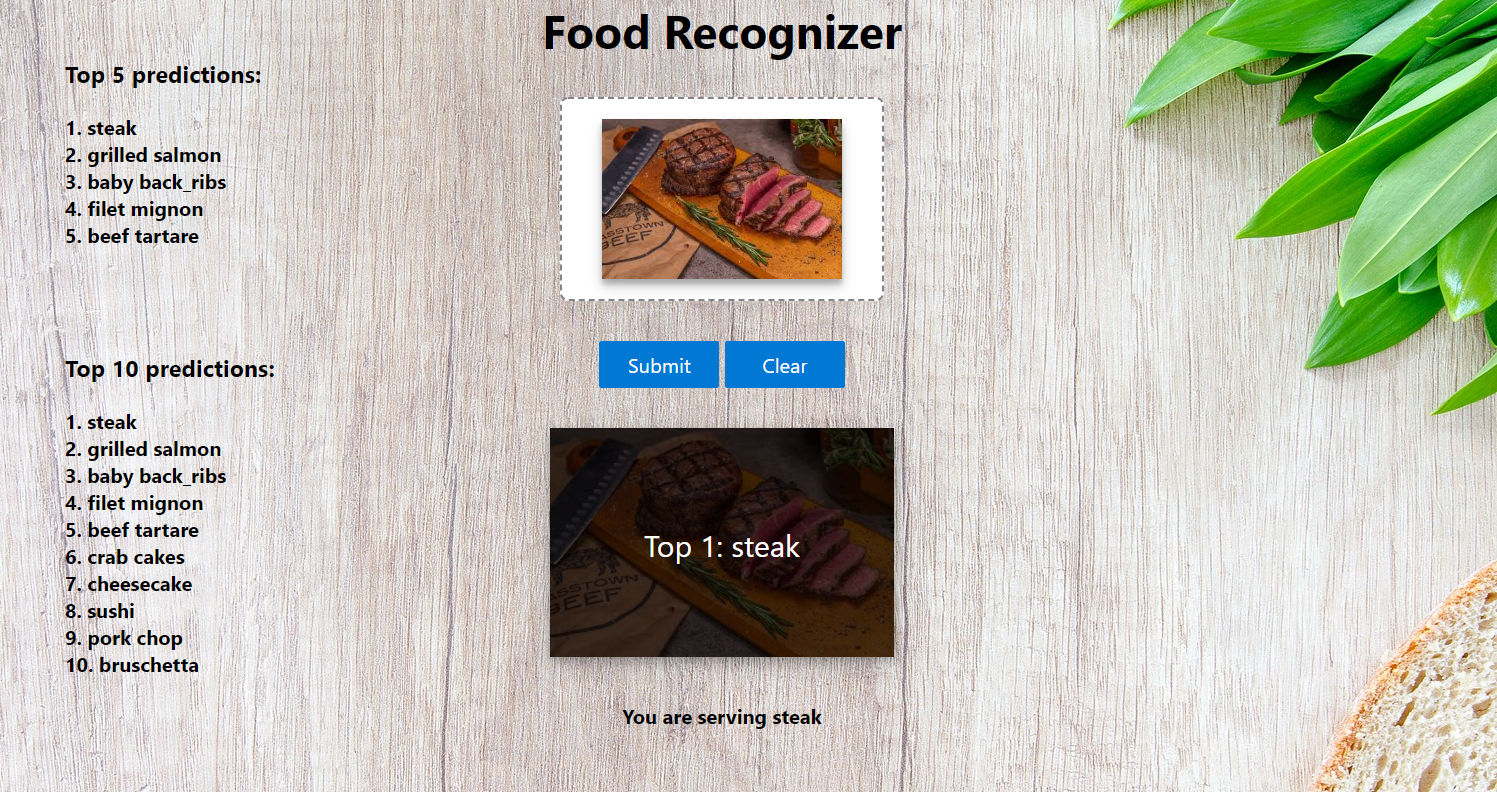
\includegraphics[width=\columnwidth]{images/3.png}}
\caption{Food Recognizer}
\label{fig:fig2}
\end{figure}

Overall, this project set out to train a network capable of classifying a food item that a user would like to donate, alleviating some tedious aspects of the donation process. This would not only create a more pleasant experience for the user who is donating, but could also encourage more donations. With the results that were achieved, our team feels strongly that we have accomplished this goal. We are successfully able to integrate our model to a web page, and the web page will later be integrated with our free food finding App, where a user will be able to simply snap pictures of the items they want to donate, and in return, the user will be provided a list to pick from that closely resembles the food they are donating. 

\bibliographystyle{IEEEtran}
\bibliography{References}

\end{document}
